\section{The Meaning of Necessity}
\label{s:semantics}

 
In this section we define {the}  \Nec specification language.  
We first define an underlying programming language, \Loo (\S \ref{sub:Loo}).
We then define an assertion language, \SpecO, which can talk about the
contents of the state, as well as about provenance, permission and
control (\S \ref{sub:SpecO}).  Finally, we define the syntax and
semantics of our full language for writing \Nec
specifications (\S \ref{s:holistic-guarantees}).


\subsection{\Loo}
\label{sub:Loo} 
%\jm[TODO: mention the type system and the restriction on external method calls]{}
%% We introduce a simple object-oriented language, \Loo, upon 
%% which our specification language sits.
 \Loo is a formal model of a {small}, imperative, sequential, 
class based, typed, object-oriented language.
%\susan[Java fields are package private not class private - are fields so important that we need to say this?]{Fields are private to the class where they are defined.}
\Loo is straightforward:
%Given its simplicity, %  the simplicity of \Loo, we do notdefine it here, instead, 
% we direct the reader to
Appendix \ref{app:loo} contains 
the full definitions.
%%and introduce here only % syntax and operational semantics.
%% the concepts relevant to the
%%treatment of the open world guarantees.
%\jm[]{\Loo fields are private in the way fields in Java are private,
%the privacy is class-wide, i.e. they may only be read or written to by 
%objects of the same class.}
\Loo is based on \LangOO 
\cite{FASE}, with some small variations, as well as 
the addition of  % while \LangOO is untyped, \Loo 
 a simple type system -- more in \ref{types}.
%has type based restrictions on external access to private data.}
%\sophiaPonder[added]{Note that the operational semantics only allows filed
%update if the receiver and the object being updated belong to the same class,
%and only allows method calls }
%
%
A \Loo state $\sigma$ consists of a 
heap $\chi$, and a  {stack $\psi$ which is a sequence of frames}.
A frame $\phi$ consists of
local variable map, and a continuation, \ie a sequence of statements to be executed.
 A statement may assign to variables, create new objects and push them to the heap, 
perform field reads and writes on objects,  or
 call methods on those objects. 

%Program 
 Modules are mappings
from class names to class definitions. 
Execution 
%takes place
is in the context of  a module $M$ and   a state $\sigma$,
%It is % Execution
 defined via unsurprising small-step semantics of the form \ \ 
   $M, \sigma \leadsto \sigma'$.
The   top frame's continuation contains the statements to be % currently being 
executed next.
 % chopped, as generic 
 % There are several properties  of \Loo that are important to the central topic of this paper. 
 
As discussed in \S \ref{s:approach}, %we are interested in 
{open world specifications need to be able to provide}
guarantees which hold
during execution of an internal, 
known, trusted module $M$ when linked together with any
unknown, untrusted, module $M'$. These guarantees need only hold 
when the external module is executing; we are not concerned if they are
temporarily broken by the internal module. Therefore, we are only interested in states where the
executing object (\prg{this}) is an external object. 
To express our focus on external states, we define the  \emph{external states semantics}, of the form 
$\reduction{M'}{M}{\sigma}{\sigma'}$, where $M'$ is the external
module, and $M$ is the internal module, and where we
collapse all internal steps into one single step.

 

\begin{definition}[External States Semantics]
\label{def:pair-reduce}
For  
% If we say "internal module", it is sounds as something makes the module be internal
  modules $M$,  $M'$, and % program
   states $\sigma$, $\sigma'$, 
we say that $\ \ \ \ \ \ \ \ \reduction{M'}{M}{\sigma}{\sigma'}\ \ \ \ \ \ \ \ $ if and only if there exist 
$n\in\mathbb{N}$, and states $\sigma_0$,...$\sigma_n$, such that
\begin{itemize}
\item
$\sigma$=$\sigma_1$, and  $\sigma'$=$\sigma_n$,
\item
$M' \circ M, \sigma_i \leadsto \sigma_{i+1}$  \ \ \ for all $i\in [0..n)$,
\item
$\class{\sigma}{\scd{\prg{this}}}, \class{\sigma'}{\scd{\prg{this}}}\in M'$,
\item
$\class{\sigma_i}{\scd{\prg{this}}} \in M$\ \ \ for all $i\in (1..n)$.
\end{itemize} 
\end{definition}
The function $\class{\sigma}{\_}$ is overloaded:
  applied to a variable, 
$\class{\sigma}{x}$  looks up the variable $x$ in the top frame of $\sigma$, and returns the 
class of the corresponding object in the  heap of $\sigma$;
%while  
applied to an address, $\class{\sigma}{\alpha}$  returns
the class of   the object referred by address $\alpha$ in the heap of $\sigma$.
 The module linking operator $\circ$, applied to two modules, $M'\circ M$, 
 combines the two modules into one module in the obvious way, provided their
domains are disjoint.
Full details in  Appendix \ref{app:loo}.
\begin{figure}[htb]
\begin{tikzpicture}[->,>=stealth',shorten >=1pt,auto,node distance=9mm,
                    thick,
                    external node/.style={circle,draw,minimum size=7mm,font=\sffamily\Large\bfseries, color=blue, fill = blue, text = black, fill opacity = 0.5},
                    internal node/.style={circle,draw,minimum size=7mm,font=\sffamily\Large\bfseries, color=orange, fill = orange, text = black, fill opacity = 0.5}]
    
	\node[external node] (a) {1};
	\node[internal node] (b) [right = of a] {2};
	\node[external node] (c) [right = of b] {3};
	\node[external node] (d) [right = of c] {4};
	\node[internal node] (e) [right = of d] {5};
	\node[internal node] (f) [right = of e] {6};
	\node[external node] (g) [right = of f] {7};
	\node[internal node] (h) [right = of g] {8};
	\node[external node] (i) [right = of h] {9}; 

	\path[every node/.style={font=\sffamily\small}]
		(a) edge[bend left] node [above] {} (b)
		(b) edge[bend left] node [above] {} (c)
		(c) edge[bend left] node [above] {} (d)
		(d) edge[bend left] node [above] {} (e)
		(e) edge[bend left] node [above] {} (f)
		(f) edge[bend left] node [above] {} (g)
		(g) edge[bend left] node [above] {} (h)
		(h) edge[bend left] node [above] {} (i);
\end{tikzpicture}
\begin{tikzpicture}[->,>=stealth',shorten >=1pt,auto,node distance=9mm,
                    thick,
                    external node/.style={circle,draw,minimum size=7mm,font=\sffamily\Large\bfseries, color=blue, fill = blue, text = black, fill opacity = 0.5},
                    internal node/.style={circle,draw,minimum size=7mm,font=\sffamily\Large\bfseries, color=orange, fill = orange, text = black, fill opacity = 0.2, draw opacity = 0.5}]
    
	\node[external node] (a) {1};
	\node[internal node] (b) [right = of a] {2};
	\node[external node] (c) [right = of b] {3};
	\node[external node] (d) [right = of c] {4};
	\node[internal node] (e) [right = of d] {5};
	\node[internal node] (f) [right = of e] {6};
	\node[external node] (g) [right = of f] {7};
	\node[internal node] (h) [right = of g] {8};
	\node[external node] (i) [right = of h] {9}; 

	\path[every node/.style={font=\sffamily\small}]
		(a) edge[bend left=46] node [above] {} (c)
		(c) edge[bend left=46] node [above] {} (d)
		(d) edge[bend left=46] node [above] {} (g)
		(g) edge[bend left=46] node [above] {} (i);
\end{tikzpicture}
   \caption{External States Semantics
     (Def. \ref{def:pair-reduce}),  %
     % 
     (A) $\exec{{\color{hotpink}M'} \circ {\color{lightseagreen}M}}{\sigma_1}{\ldots}\leadsto \sigma_9$\ \ \and \ \ \ 
     (B) $\reduction{{\color{hotpink}M'}}{{\color{lightseagreen}M}}{\sigma_2}{\ldots}\leadsto \sigma_9$, \ \ \ 
     \\
     where $\class{{\color{lightseagreen}\sigma_1}}{\scd{\prg{this}}}$,$\class{{\color{lightseagreen}\sigma_3}}{\scd{\prg{this}}}$,$\class{{\color{lightseagreen}\sigma_4}}{\scd{\prg{this}}}$,$\class{{\color{lightseagreen}\sigma_7}}{\scd{\prg{this}}}$,$\class{{\color{lightseagreen}\sigma_8}}{\scd{\prg{this}}}\in {\color{lightseagreen}M}$,\\
     and where $\class{{\color{hotpink}\sigma_2}}{\scd{\prg{this}}},\class{{\color{hotpink}\sigma_5}}{\scd{\prg{this}}} 
     \class{{\color{hotpink}\sigma_6}}{\scd{\prg{this}}},\class{{\color{hotpink}\sigma_9}}{\scd{\prg{this}}}\in {\color{hotpink}M'}$.
    %  (c) $\reduction{{\color{orange}M'}}{{\color{blue}M}}{\sigma_1}{\ldots}\leadsto \sigma_8$
    }
   \label{fig:VisibleStates}
 \end{figure}
 
Fig. \ref{fig:VisibleStates} inspired by \citeasnoun{FASE} provides a simple graphical description of 
our external states semantics: (A) is the ``normal'' execution after 
linking two modules into one: \ $M' \circ M, ... \leadsto ...$ whereas (B) is the
 external states execution when $M'$ is external,\   $\reduction{M'}{M}{...}{...}$.
Note that whether a module is external or internal depends on %our
perspective -- nothing in a module itself renders it internal or external. For example, in
 $\reduction{M_1}{M_2}{...}{...}$ the external module is $M_1$,
  while in  $\reduction{M_2}{M_1}{...}{...}$  the external module is $M_2$.

We  use the notation\ \  $\reductions{M'}{M}{\sigma}{\sigma'}$ \ 
to denote zero or more  steps starting at state $\sigma$ and ending at state $\sigma'$, in the context of internal module 
$M$ and external module $M'$.
 %Not only are we unconcerned 
%with internal states,  we are also unconcerned with  states which cannot ever arise from execution.
We are concerned neither with internal states nor states that can never arise.
{A state $\sigma$ is \emph{arising},}  written $\arising{M'}{M}{\sigma}$, {if it  may arise by external states} execution
starting at some initial configuration:



\begin{definition}[Arising  States]
\label{def:arising}
For   modules $M$ and  $M'$, a % program
 state $\sigma$ is 
called an \emph{arising} state, formally \ \ \ $\arising{M'}{M}{\sigma}$,\ \ \ 
if and only if there exists some $\sigma_0$ such that $\initial{\sigma_0}$ and
$\reductions{M'}{M}{\sigma_0}{\sigma}$.
\end{definition}

An \emph{Initial} state's heap
contains a single object of class \prg{Object}, and
its  stack   consists of a single frame, whose local variable map is a
mapping from \prg{this} to the single object, and whose continuation is  any statement.
(See Definitions \ref{def:initial} and \ref{def:arising}).


\paragraph{Applicability} 
{While our work is based on 
  a simple, imperative, typed, object oriented}
language with unforgeable addresses and private fields, we believe
 that % our approach
 it is applicable to several programming paradigms, and 
 that   unforgeability and privacy
 can be replaced 
 by lower level mechanisms such as capability machines \cite{vanproving,davis2019cheriabi}.

\subsection{\SpecO}
\label{sub:SpecO}

\SpecO is a subset of the \emph{Chainmail} assertions language, \ie
a basic assertion language extended with
object-capability assertions. 


\subsubsection{Syntax of \SpecO}
The syntax of \SpecO   is given in
Definition \ref{f:chainmail-syntax}.
An assertion may be an expression,   a query of the defining class of
  an object, the usual connectives and quantifiers, along 
with three non-standard assertion forms:
(1) \emph{Permission} and (2) \emph{Provenance}, inspired by the capabilities literature, and
(3) \emph{Control} which allows tighter  characterisation of the cause of effects --  
useful for the specification of large APIs.
\begin{itemize}
\item
\emph{Permission} ($\access{x}{y}$):  
  $x$ has access to $y$.
\item
{\emph{Provenance}} ($\internal{x}$ and $\external{y}$):   $x$ is internal, and $y$ is external.
\item
\emph{Control} ($\calls{x}{y}{m}{\overline{z}}$): 
$x$ calls method $m$ on object $y$ with arguments $\overline{z}$.
\end{itemize}


\begin{definition}
Assertions ($A$) in
\SpecO are defined as follows:

\label{f:chainmail-syntax}
 \[
\begin{syntax}
\syntaxElement{A}{}
		{
		\syntaxline
				{e}
				{e : C}
				{\neg A}
				{A\ \wedge\ A}
				{A\ \vee\ A}
				{\all{x}{A}}
				{\ex{x}{A}}
		\endsyntaxline
		}
		{
		\syntaxline
				{\access{x}{y}}
				{\internal{x}}
				{\external{x}}
%		\endsyntaxline
%		}
%		{
%		\syntaxline
				{\calls{x}{y}{m}{\overline{z}}}
		\endsyntaxline
		}
\endSyntaxElement\\
\end{syntax}
\]


\end{definition}



\subsubsection{Semantics of \SpecO}
The semantics of \SpecO   
is given in Definition \ref{def:chainmail-semantics}. 
We   use the evaluation relation, $\eval{M}{\sigma}{e}{v}$,
which says that the expression $e$ evaluates
to value $v$ in the context of state $\sigma$ and module $M$.
Note that expressions in \Loo may be recursively defined, and thus evaluation 
need not always % may not necessarily 
 terminate. Nevertheless, the logic of $A$ remains classical because recursion is restricted
to expressions, and not generally to assertions.
We have taken this approach from \citeasnoun{FASE}, which also contains a mechanized Coq proof that assertions are classical \cite{coqFASE}.
%  The full
The semantics of $\hookrightarrow$ are unsurprising (see Fig.\ref{f:evaluation}).

Shorthands: 
 $\interpret{\phi}{x} = v$  means that $x$ maps to
value $v$ in the local variable map of frame $\phi$, $\interpret{\sigma}{x} = v$ means that $x$ 
maps to $v$ in the top most frame of $\sigma$'s stack, and $\interpret{\sigma}{x.f} = v$
has the obvious meaning. The terms $\sigma.\prg{stack}$,  
%resp. 
$\sigma.\prg{contn}$, 
%resp. 
$\sigma.\prg{heap}$     mean the stack, 
%resp. 
the continuation at the
top frame of $\sigma$, %resp. 
and the heap of $\sigma$.
The term $\alpha\!\in\!\sigma.\prg{heap}$ means that $\alpha$ is in the domain of the heap of $\sigma$, and \emph{$x$ fresh in $\sigma$} means that 
$x$ isn't in the variable map of the top frame of $\sigma$, 
while the substitution  $\sigma[x \mapsto \alpha]$ is applied to the top frame of $\sigma$.
$C\in M$ means that class $C$ is in the domain of module $M$. 

\begin{definition}[Satisfaction % of \SpecO 
of Assertions by a module and a state] 
\label{def:chainmail-semantics}
We define satisfaction of an assertion $A$ by a % program 
state $\sigma$ with 
 module $M$ as:
\begin{enumerate}
\item
\label{cExpr}
$\satisfiesA{M}{\sigma}{e}$ \ \ \ iff \ \ \  $\eval{M}{\sigma}{e}{\true}$
\item
\label{cClass}
$\satisfiesA{M}{\sigma}{e : C}$ \ \ \ iff \ \ \  $\eval{M}{\sigma}{e}{\alpha}$ \textit{and} $\class{\sigma}{\alpha} = C$
\item
$\satisfiesA{M}{\sigma}{\neg A}$ \ \ \ iff \ \ \  ${M},{\sigma}\nvDash{A}$
\item
$\satisfiesA{M}{\sigma}{A_1\ \wedge\ A_2}$ \ \ \ iff \ \ \  $\satisfiesA{M}{\sigma}{A_1}$ and 
$\satisfiesA{M}{\sigma}{A_2}$
\item
$\satisfiesA{M}{\sigma}{A_1\ \vee\ A_2}$ \ \ \ iff \ \ \  $\satisfiesA{M}{\sigma}{A_1}$ or 
$\satisfiesA{M}{\sigma}{A_2}$
\item
$\satisfiesA{M}{\sigma}{\all{x}{A}}$ \ \ \ iff \ \ \  
$\satisfiesA{M}{\sigma[x \mapsto \alpha]}{A}$, \ 
\ \ \ for some $x$ fresh in $\sigma$, and for all $\alpha\!\in\!\sigma.\prg{heap}$.
\item
$\satisfiesA{M}{\sigma}{\ex{x}{A}}$ \ \ \ iff \ \ \  
$\satisfiesA{M}{\sigma[x \mapsto \alpha]}{A}$, \ 
\ \ for some $x$ fresh in $\sigma$, and for some $ \alpha\!\in\!\sigma.\prg{heap}$. 
\item
\label{cAccess}
$\satisfiesA{M}{\sigma}{\access{x}{y}}$ \ \ \ iff \ \ \  
\begin{enumerate}
\item
\label{c1}
$\interpret{\sigma}{x.f}={\interpret{\sigma}{y}}$ for some $f$, \\
  or
\item
\label{c2}
{$\interpret{\sigma}{x}=\interpret{\phi}{\prg{this}}$}, {$\interpret{\sigma}{y}=\interpret{\phi}{z}$}, and $z\ \in\ \phi.\prg{contn}$\ \ \ \
for some variable $z$, and some frame $\phi$ in $\sigma.
\prg{stack}$.
\end{enumerate}
\item
\label{cInternal}
$\satisfiesA{M}{\sigma}{\internal{x}}$ \ \ \ iff \ \ \  
$\textit{classOf}(\sigma,x) \in M$
\item
\label{cExternal}
$\satisfiesA{M}{\sigma}{\external{x}}$ \ \ \ iff \ \ \  
$\textit{classOf}(\sigma,x) \not\in M$
\item
\label{cCall}
$\satisfiesA{M}{\sigma}{\calls{x}{y}{m}{z_1, \ldots, z_n}}$ \ \ \ iff \ \ \ 
\begin{enumerate}
\item
$\sigma.\prg{contn} = (w := y'.m(z'_1,\ldots,z'_n)\scd{; s})$,\ \ for some 
variable $w$, and some statement $s$,
\item
$\satisfiesA{M}{\sigma}{x = \prg{this}}$
\ \ and \ \ 
$\satisfiesA{M}{\sigma}{y = y'}$,
\item
$\satisfiesA{M}{\sigma}{z_i = z'_i}$\ \ \ for all $1\!\leq i\!\leq n$
\end{enumerate}
\end{enumerate}
\end{definition}

 
The assertion ${\access{x}{y}}$ (defined in  \ref{cAccess})
requires  that $x$ has access to $y$
either through a field of $x$ (case \ref{c1}),
or through some call in the stack, where $x$ is the receiver and $y$ is one of the
arguments (case \ref{c2}).
{Note that access is not deep, and only refers to objects that 
an object has direct access to via a field or within the context of a current scope. 
%A transitive definition of access would not be useful in specifying safe and robust software.
 The restricted form of access used in \Nec specifically captures a crucial property of robust programs in the open world: access to an object does not imply access to that object's internal data. For example, an object may have access to an account \prg{a}, but a safe implementation of the account would never allow that object to leverage that access to gain direct access to {\prg{a.pwd}}}.
 %Necessity is thus concerned with if and how objects are able to gain direct access to an object, and not deep, transitive access. Indeed, if access were defined transitively, then many objects would be defined as having access to objects that they could not gain a direct reference to, and as such render <x access y> as almost meaningless, and any safety specifications written using access to be prohibitively restrictive.
 
 The assertion %$\satisfiesA{M}{\sigma}
 ${\calls{x}{y}{m}{z_1, \ldots, z_n}}$  (defined in \ref{cCall}) 
requires that the current receiver (\prg{this}) is $x$, and that it calls the method $m$ on $y$ with
 arguments $z_1$, ... $z_n$ -- It does \emph{not} mean  that somewhere in the 
 call stack there exists a call from $x$ to $y.m(...)$. 
 Note that in most cases, satisfaction of an assertion not only depends on the state $\sigma$, but 
also depends on the module in the case of expressions (\ref{cExpr}), class membership
(\ref{cClass}), and internal or external provenance (\ref{cInternal} and \ref{cExternal}).


We now define what it means for a module to satisfy an assertion:
 $M$ satisfies  $A$ if any state arising from external steps execution of that
module with any other external module  satisfies $A$. 
 
\begin{definition} [Satisfaction % of \SpecO 
of Assertions
by a module] 
\label{def:mdl-sat}
For a module $M$ and assertion $A$, we say that\ \  $\satisfies{M}{A}$ \ \ if and only if 
for all modules $M'$, and all $\sigma$, if $\arising{M'}{M}{\sigma}$, then $\satisfiesA{M}{\sigma}{A}$.
\end{definition}

 
In the current work we assume the existence of a proof system that judges
$\proves{M}{A}$, to prove  satisfaction of assertions. 
 We will not define such a judgement, but will rely on its existence {later on for} Theorem \ref{thm:soundness}.
We define soundness of such a judgement in the usual way:

\begin{definition}[Soundness of \SpecO Provability]
\label{ax:specW-prove-soundness}
A judgement of the form {$\proves{M}{A}$} is \emph{sound}, if for all
 modules $M$ and assertions $A$, \ if $\proves{M}{A}$ then $\satisfies{M}{A}$.
\end{definition}

 
\subsubsection{Inside}

We define
a final shorthand 
predicate $\wrapped{\prg{o}}$ which states 
that only \internalO objects have access to \prg{o}.
The object \prg{o} may be either \internalO or \externalO.
\begin{definition}[Inside]
$\wrapped{o}\ \triangleq\ \all{x}{\access{x}{o}\ \Rightarrow\ \internal{x}} $ 
\end{definition}

 
\inside is a very useful concept. For example, the balance of an account whose
  password is \inside  will not decrease in the next step.
  Often, API implementations contain objects whose capabilities, while  crucial for the implementation, if exposed,
would break the intended guarantees of the API. Such objects need to remain \inside - see
such an example in Section \ref{s:examples}. 
 


\subsection {\Nec operators}
\label{s:holistic-guarantees}

The \Nec specification language extends \SpecO with our three novel 
 \emph{necessity operators}:

\begin{description}
\item[Only If]
[$\onlyIf{A_1}{A_2}{A}$]: If an arising % program
  state satisfies $A_1$, and after some execution, a state % program 
 satisfying $A_2$ is reached, 
then the original  
state must have also satisfied $A$.
 %e.g. if the balance of a bank account changes over time, then there must be some external object in the current 
%program  state that has access to the account's password.
% \paragraph{Single-Step Only If}
\item[Single-Step Only If]
[$\onlyIfSingle{A_1}{A_2}{A}$]: If an arising %program
  state satisfies $A_1$, and after a single step of execution, a state satisfying $A_2$ is reached, 
then the original %program 
state must have also satisfied $A$.
%e.g. if the balance of a bank account changes over a single execution step, then that execution step must be a method call to the bank \prg{transfer} method.

%\paragraph{Only Through}
\item[Only Through]
[$\onlyThrough{A_1}{A_2}{A}$]: If an arising %program 
 state satisfies $A_1$, and after some execution, a state satisfying $A_2$ is reached, then  execution must have passed through some \emph{intermediate} state satisfying $A$ 
% e.g. if the balance of an account changes over time, then the bank's \prg{transfer} method must have been called 
% in some intermediate state. Note 
--  the   \emph{intermediate} state % state where $A$ is true
satisfying $A$ might be the \emph{starting}  
state, the \emph{final} state, or any state in between.
\end{description}


\label{sec:adapt:motivate}
\noindent Necessity operators can explicitly constrain two or even three states,
and implicitly constrain many states in between. The following 
 specification  \Sadapt 
 says that for an account's balance to go  
 from 350 in one state down to 250 some subsequent state, 
% in \emph{one} step,
 \prg{transfer} must have been called on that account in between:
%
% SD we write all specs in 2 lines only
\begin{lstlisting}[language = Chainmail, mathescape=true, frame=lines]
$\text{\Sadapt}$  $\triangleq$  from a:Account $\wedge$ a.balance == 350  to a.balance == 250
                  onlyThrough $\exists \prg{o},\prg{o'},\prg{o''}.\calls{\prg{o}}{\prg{a}}{\prg{transfer}}{\prg{o'},\prg{o''}}$
\end{lstlisting}
%
\Sadapt  refers to {two or even three} different states: at 
the start,  whenever the balance of \prg{a} is \prg{350}, and after any number of steps
whenever the balance of \prg{a} is \prg{250}. The specification requires
that such a change can only be caused by a call to \prg{transfer} {on \prg{a}}:
that call could be in the current (starting) state,
  in which case
 presumably the balance will be \prg{250} in the immediately following state,
or within any number of intervening states.




\paragraph{Relationship between Necessity Operators}
The three \Nec \ operators
are related by generality. 
%An 
 \emph{Only If} ($\onlyIf{A_1}{A_2}{A}$) implies
  \emph{Single-Step Only If} ($\onlyIfSingle{A_1}{A_2}{A}$), since if $A$ is 
a necessary precondition for multiple steps, then it must be a necessary 
precondition for a single step. 
 \emph{Only If} also implies 
an \emph{Only Through}, where the intermediate state is the starting state
of the execution.  There is no further relationship between 
\emph{Single-Step Only If} and \emph{Only Through}.


\paragraph{Relationship with Temporal Logic}
Two of the three \Nec operators can be expressed in traditional
  temporal logic: 
  ${\onlyIf{A_1}{A_2}{A}}$
can be expressed  %%put in to get better line breaks
 as 
 $A_1\ \wedge\ \Diamond A_2\ \longrightarrow\ A$, and
 $\onlyIfSingle{A_1}{A_2}{A}$
can be expressed  %%put in to get better line breaks
 as $\ A_1\ \wedge\ \bigcirc A_2\ \longrightarrow\ A$
 (where $\Diamond$ denotes any future state,  and
 $\bigcirc$ denotes the next state).
 Critically, 
$\onlyThrough{A_1}{A_2}{A}$ cannot be encoded in temporal logics
  without ``nominals'' (explicit state references), because the state where $A$ 
 holds must be between the state where $A_1$ holds, and the state
 where $A_2$ holds; and this must be so on \emph{every} execution path
 from $A_1$ to  $A_2$ \cite{hybridLogic2021,nominal-seplogic2020}.
 TLA+, for example, cannot describe ``only through'' conditions
 \cite{tlabook}, but we have found ``only through'' conditions critical
 to our proofs. 

  

\subsubsection{Semantics of \Nec Specifications}


We    define  when a module $M$ satisfies  specifications $S$, written as $M \vDash S$, 
by cases over the four possible syntactic forms: 


\begin{definition}[\Nec Syntax]

\footnotesize
\[
\begin{syntax}
\syntaxElement{S}{}
		{
		\syntaxline
				{A}
				{\onlyIf{A_1}{A_2}{A_3}}
				{\onlyThrough{A_1}{A_2}{A_3}}
		\endsyntaxline
		}
		{
		\syntaxline
				{\onlyIfSingle{A_1}{A_2}{A_3}}
		\endsyntaxline
		}
\endSyntaxElement\\
\end{syntax}
\]
%\caption{Syntax of \Chainmail Necessity Specifications}
\label{f:holistic-syntax}
\end{definition}
%\end{figure}
\normalsize




\noindent
\begin{definition}[\Nec Semantics]
\label{def:necessity-semantics}
For any assertions   $A_1$, $A_2$, and $A$,  we define \\


$\bullet$ \ $\satisfies{M}{{A}}$ \ \ \ iff\ \ \ for all $M'$, $\sigma$,\ if $\arising{M'}{M}{\sigma}$, then $\satisfiesA{M}{\sigma}{A}$. (see Def. \ref{def:mdl-sat})\\

%$\bullet$ \ $\satisfies{M}{{A}}$ \ \ \ as defined in \ref{def:mdl-sat} \\

$\bullet$ \ $\satisfies{M}{\onlyIf {A_1}{A_2}{A}}$ \ \ iff\ \  for all $M'$, $\sigma$, $\sigma'$, such that $\arising{M'}{M}{\sigma}$; \\ % and\\

\begin{tabular}{lr}
$\;\;\;\;$- $\satisfiesA{M}{\sigma}{A_1}$  & \rdelim\}{3}{3mm}[$\;\;\;\Rightarrow\;\;\;$  $\satisfiesA{M}{\sigma}{A}$] \\
$\;\;\;\;$- $\satisfiesA{M}{\sigma' \triangleleft \sigma}{A_2}$   \\
$\;\;\;\;$- $\reductions{M'}{M}{\sigma}{\sigma'}$   \\
\end{tabular}\\ 

$\bullet$ \  $\satisfies{M}{\onlyIfSingle {A_1}{A_2}{A}}$\ \ iff\ \   for all $M'$, $\sigma$,   $\sigma'$, such that $\arising{M'}{M}{\sigma}$: \\

\begin{tabular}{lr}
$\;\;\;\;$- $\satisfiesA{M}{\sigma}{A_1}$  & \rdelim\}{3}{3mm}[$\;\;\;\Rightarrow\;\;\;$  $\satisfiesA{M}{\sigma}{A}$] \\
$\;\;\;\;$- $\satisfiesA{M}{\sigma' \triangleleft \sigma}{A_2}$   \\
$\;\;\;\;$- $\reduction{M'}{M}{\sigma}{\sigma'}$   \\
\end{tabular}\\ 
  
$\bullet$ \  $\satisfies{M}{\onlyThrough {A_1}{A_2}{A}}$ \ \ iff\ \  for all $M'$, $\sigma_1$,   $\sigma_n$, such that $\arising{M'}{M}{\sigma_1}$: \\

\begin{tabular}{lr}
$\;\;\;\;$- $\satisfiesA{M}{\sigma_1}{A_1}$  & 
\rdelim\}{3}{3mm}%[\makecell{Some really \\ longer text}]
[$\;\;\;\Rightarrow\;\;\;$\pbox{9cm}{$\forall \sigma_2, \ldots, \sigma_{n-1}$.  \\ 
(\ \ $\forall i\!\in\![1..n).\ \reduction{M'}{M}{\sigma_i}{\sigma_{i+1}}$   \ $\Rightarrow$
$\exists i\!\in\![1..n]. \  \satisfiesA{M}{\sigma_i \triangleleft \sigma_1}{A}$ \ \ )   }] \\
$\;\;\;\;$- $\satisfiesA{M}{\sigma_n\triangleleft \sigma\sd{_1}}{A_2}$   \\
$\;\;\;\;$- $\reductions{M'}{M}{\sigma\sd{_1}}{\sigma_n}$   \\
\end{tabular} 
\end{definition} 

\subsubsection{Adaptation}
\label{sub:adapt:full}

The definition of the necessity operators
(Definition~\ref{def:necessity-semantics}) is straightforward, apart from one
quirk: we write $\adapt  {\sigma'}{\sigma}$  (best read as ``$\sigma'$ seen
from $\sigma$'', although one recalcitrant author prefers ``$\sigma'$
adapted to $\sigma$'') to deal with the fact that necessity operators
can involve several states. To see the problem, 
consider a na{\"\i}ve approach to giving semantics to \Sadapt:  if
$..,\sigma  \models \prg{a.balance==350}$, 
and  $.., \sigma  \leadsto^* \sigma'$ and $\sigma' \models \prg{a.balance==250}$,
{then  \Sadapt mandates that between $\sigma$ and $\sigma'$ there was a
call to   \prg{a.transfer}.}
But if $\sigma$ happened to have another account \prg{a1} with balance
\prg{350}, and if we reach $\sigma'$ from $\sigma$ by executing \prg{a1.transfer(}$..,..$\prg{); a=a1}, then we would 
reach a $\sigma'$ % SD chop as superfluous where $\sigma'\models \prg{a.balance==250}$
\emph{without} \prg{a.transfer} having been called: indeed, without the
account \prg{a} from $\sigma$  having changed at all!
(Haskell programmers will probably feel at home here).  


This is the remit of the adaptation operator: when we consider the
future state, we must ``see it from'' the perspective of the current
state; the binding for variables such as \prg{a} must be from the
current state, even though we may have assigned to them in the mean
time.  Thus, $\adapt {\sigma'} {\sigma}$ keeps the heap from $\sigma'$,
and renames the variables
in the top stack frame of  $\sigma'$ so that all variables defined in $\sigma$ have the same 
bindings
%?  ($\adapt {\sigma'} {\sigma}$)
as in   $\sigma$; the continuation must be adapted similarly (see
Fig.~\ref{fig:Adaptation}).
%
%
\begin{figure}[htbp]
\begin{tabular}{clclc}
 \begin{minipage}{0.27\textwidth}
 $\sigma:$\\
% ~ \\
 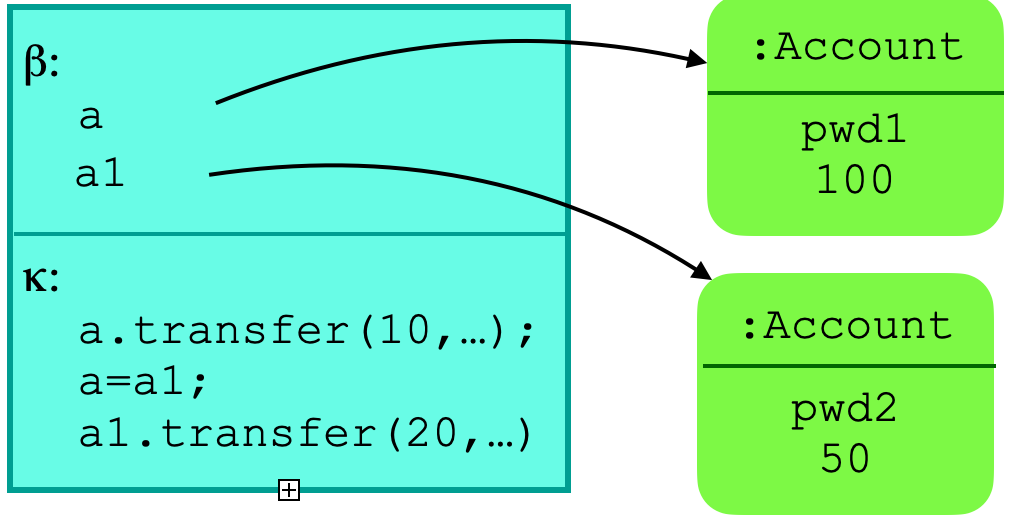
\includegraphics[width=\linewidth]{diagrams/adapt1.png}
   \end{minipage}
 & \ \ \ &
 \begin{minipage}{0.27\textwidth}
  $\sigma':$\\
 % ~ \ \\
  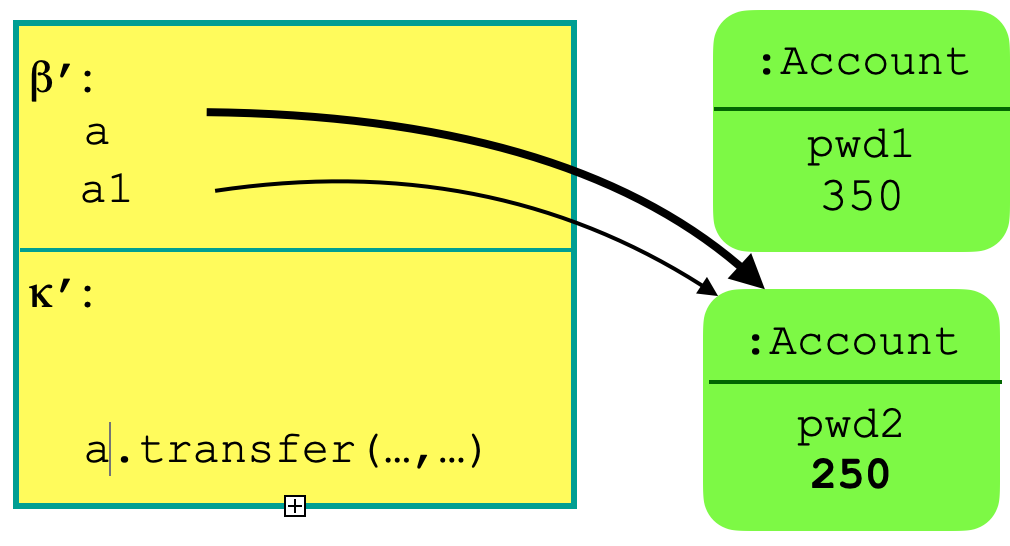
\includegraphics[width=\linewidth]{diagrams/adapt2.png}
   \end{minipage}
   & \ \ \  &
    \begin{minipage}{0.27\textwidth}
$\adapt {\sigma'}{\sigma}:$\\
% ~ \\
  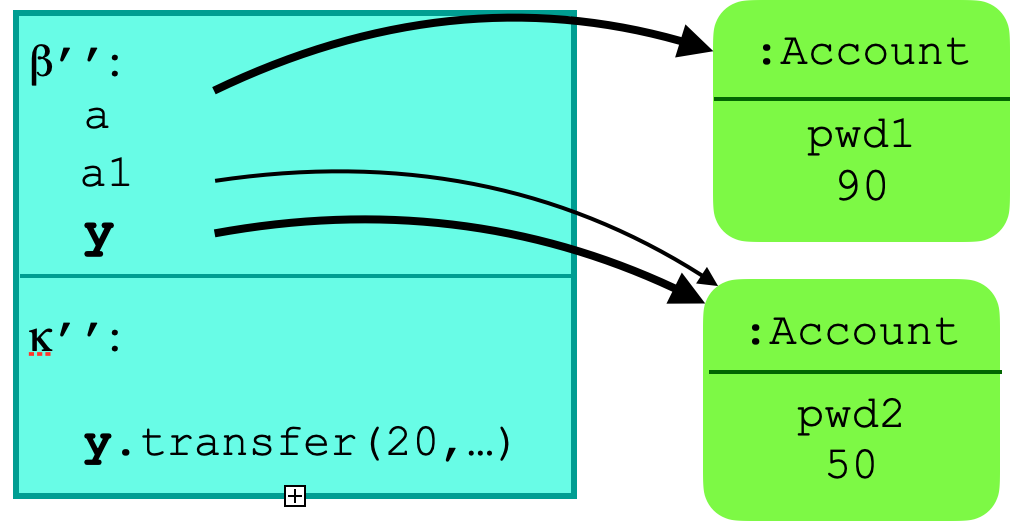
\includegraphics[width=\linewidth]{diagrams/adapt3.png}
   \end{minipage}
\end{tabular}
\caption{Illustrating adaptation
}
\label{fig:Adaptation}
\end{figure}




Under adaptation, the semantics of \Sadapt is:\  if $..,\sigma \models \prg{a.balance==350}$,
and  $.., \sigma \leadsto^* \sigma'$ and $..., \boldsymbol{\adapt {\sigma'}{\sigma}} \models \prg{a.balance==250}$,
%then $\sigma_1$'s continuation starts with a call to 
{some intermediate state's continuation contains a call to \prg{a.transfer}};
where every reference to \prg{a} in any part of the necessity operator
refers to the object bound to that variable in the initial state.
%
Fig.~\ref{fig:Adaptation} illustrates this semantics. In state $\sigma$ the variable \prg{a} points to an \prg{Account}
object with password \prg{pwd1}, and balance \prg{350},  the variable \prg{a1} points to an \prg{Account}
object with password \prg{pwd2}, and balance \prg{350}, and the continuation is \prg{a1.transfer(}$..,..$\prg{);} \prg{a=a1;}
\prg{a.transfer(}$..,..$\prg{);}. 
We reach $\sigma'$ by executing the first two statements from the continuation.
{Thus,  ${\adapt {\sigma'}{\sigma}}\not\models \prg{a.balance==250}$}.
Moreover, in $\adapt {\sigma'}{\sigma}$ we introduce the fresh variables \prg{y} and \prg{y1}, and replace \prg{a} and
\prg{a1} by \prg{y} and \prg{y1} in the continuation.
This gives that ${\adapt {\sigma'}{\sigma}} \models \calls {\_} {\prg{a1}} {\prg{transfer}} {...}$ and  ${\adapt {\sigma'}{\sigma}}\not\models \calls {\_} {\prg{a}} {\prg{transfer}} {...}$.

 

Definition~\ref{d:adapt} gives the full definition of the $\adapt{}{}$ operator
(equivalent to the \emph{adaptation} operator from \cite{FASE}).
We introduce fresh variables  $\overline{y}$ -- as many as in the $\sigma'$ top frame variable map
-- $dom(\beta')=\overline{x}$,  and $|\overline{y}| = |\overline{x}|$.  
We extend $\sigma$'s variable map ($\beta$), so that it also maps $\overline{y}$ 
in the way that  $\sigma'$'s variable map ($\beta'$) maps its local variables -- $\beta'' =  \beta[\overline{y} \mapsto  {\beta'(\overline{x})}]$. We rename $\overline{x}$   in $\sigma'$ continuation
to $\overline{y}$ --  $\kappa''=[\overline{y}/\overline{x}]\kappa'$.

 
 
\begin{definition}
\label{d:adapt}
For any states $\sigma$, $\sigma'$, heaps $\chi$, $\chi'$, %frames $\phi$, $\phi'$, 
variable maps $\beta$, $\beta'$, 
and continuations $\kappa$, $\kappa'$, such that 
$\sigma$=$(\chi,(\beta,\kappa):\psi)$, and $\sigma$=$(\chi',(\beta',\kappa'):\psi')$, we define 
\begin{itemize}
\item $\adapt{\sigma'}{\sigma} \triangleq (\chi', (\beta'',\kappa'') : \psi')$ \\
where there exist variables $\overline{y}$ such that
\begin{itemize}
\item
$\beta'' =  \beta[\overline{y} \mapsto  {\beta'(\overline{x})}]$, \ and\  $\kappa''=[\overline{y}/\overline{x}]\kappa'$
\item
$dom(\beta')=\overline{x}$,  and $|\overline{y}| = |\overline{x}|$,\  and\  $\overline{y}$ are fresh in $\beta$ and $\beta'$.
\end{itemize}
\end{itemize}
\end{definition}



{Strictly speaking, $\adapt {}{}$  does not define one  unique state: Because  variables $\overline{y}$ 
are arbitrarily chosen,   $\adapt {}{}$ describes an infinite set of states. These states satisfy the same assertions
and therefore are   equivalent with each 
other.
This is why it is sound to  use $\adapt {}{}$  as an operator, rather than as a set.
}

